\documentclass{article}
\usepackage{graphicx}
\usepackage{wrapfig}
\usepackage{subcaption}
\usepackage[margin=1in]{geometry}
\usepackage{amsmath} % or simply amstext
\usepackage{siunitx}
\usepackage{booktabs}
\usepackage[export]{adjustbox}
\newcommand{\angstrom}{\textup{\AA}}
\usepackage{cleveref}
\usepackage{booktabs}
\usepackage{gensymb}
\usepackage{float}

\title{Understanding missing diffraction reflections}

\begin{document}

\graphicspath{{./figures/}}  % put all the figures here
\maketitle

Initial configurations are built in two ways: Parallel displaced and Sandwiched
(Figure ~\ref{fig:initial_configs}).  The simulated diffraction patterns for
equilibrated systems started in each configuration at 300 K are shown in Figure
~\ref{fig:xrd}. We observe stronger features in the alkane chain region when
the temperature is lowered to 280K (Figure~\ref{fig:xrd_280}). At both
temperatures we are missing what appears to be a subharmonic located at
($q_r=0$,$q_z=0.85$) in the experimental pattern. We would like to know 
why it doesn't appear -- whether it has something to do with our system
or the math behind the simulated structure factor itself. 

\begin{figure}
        \begin{subfigure}{0.475\textwidth}
                \centering
                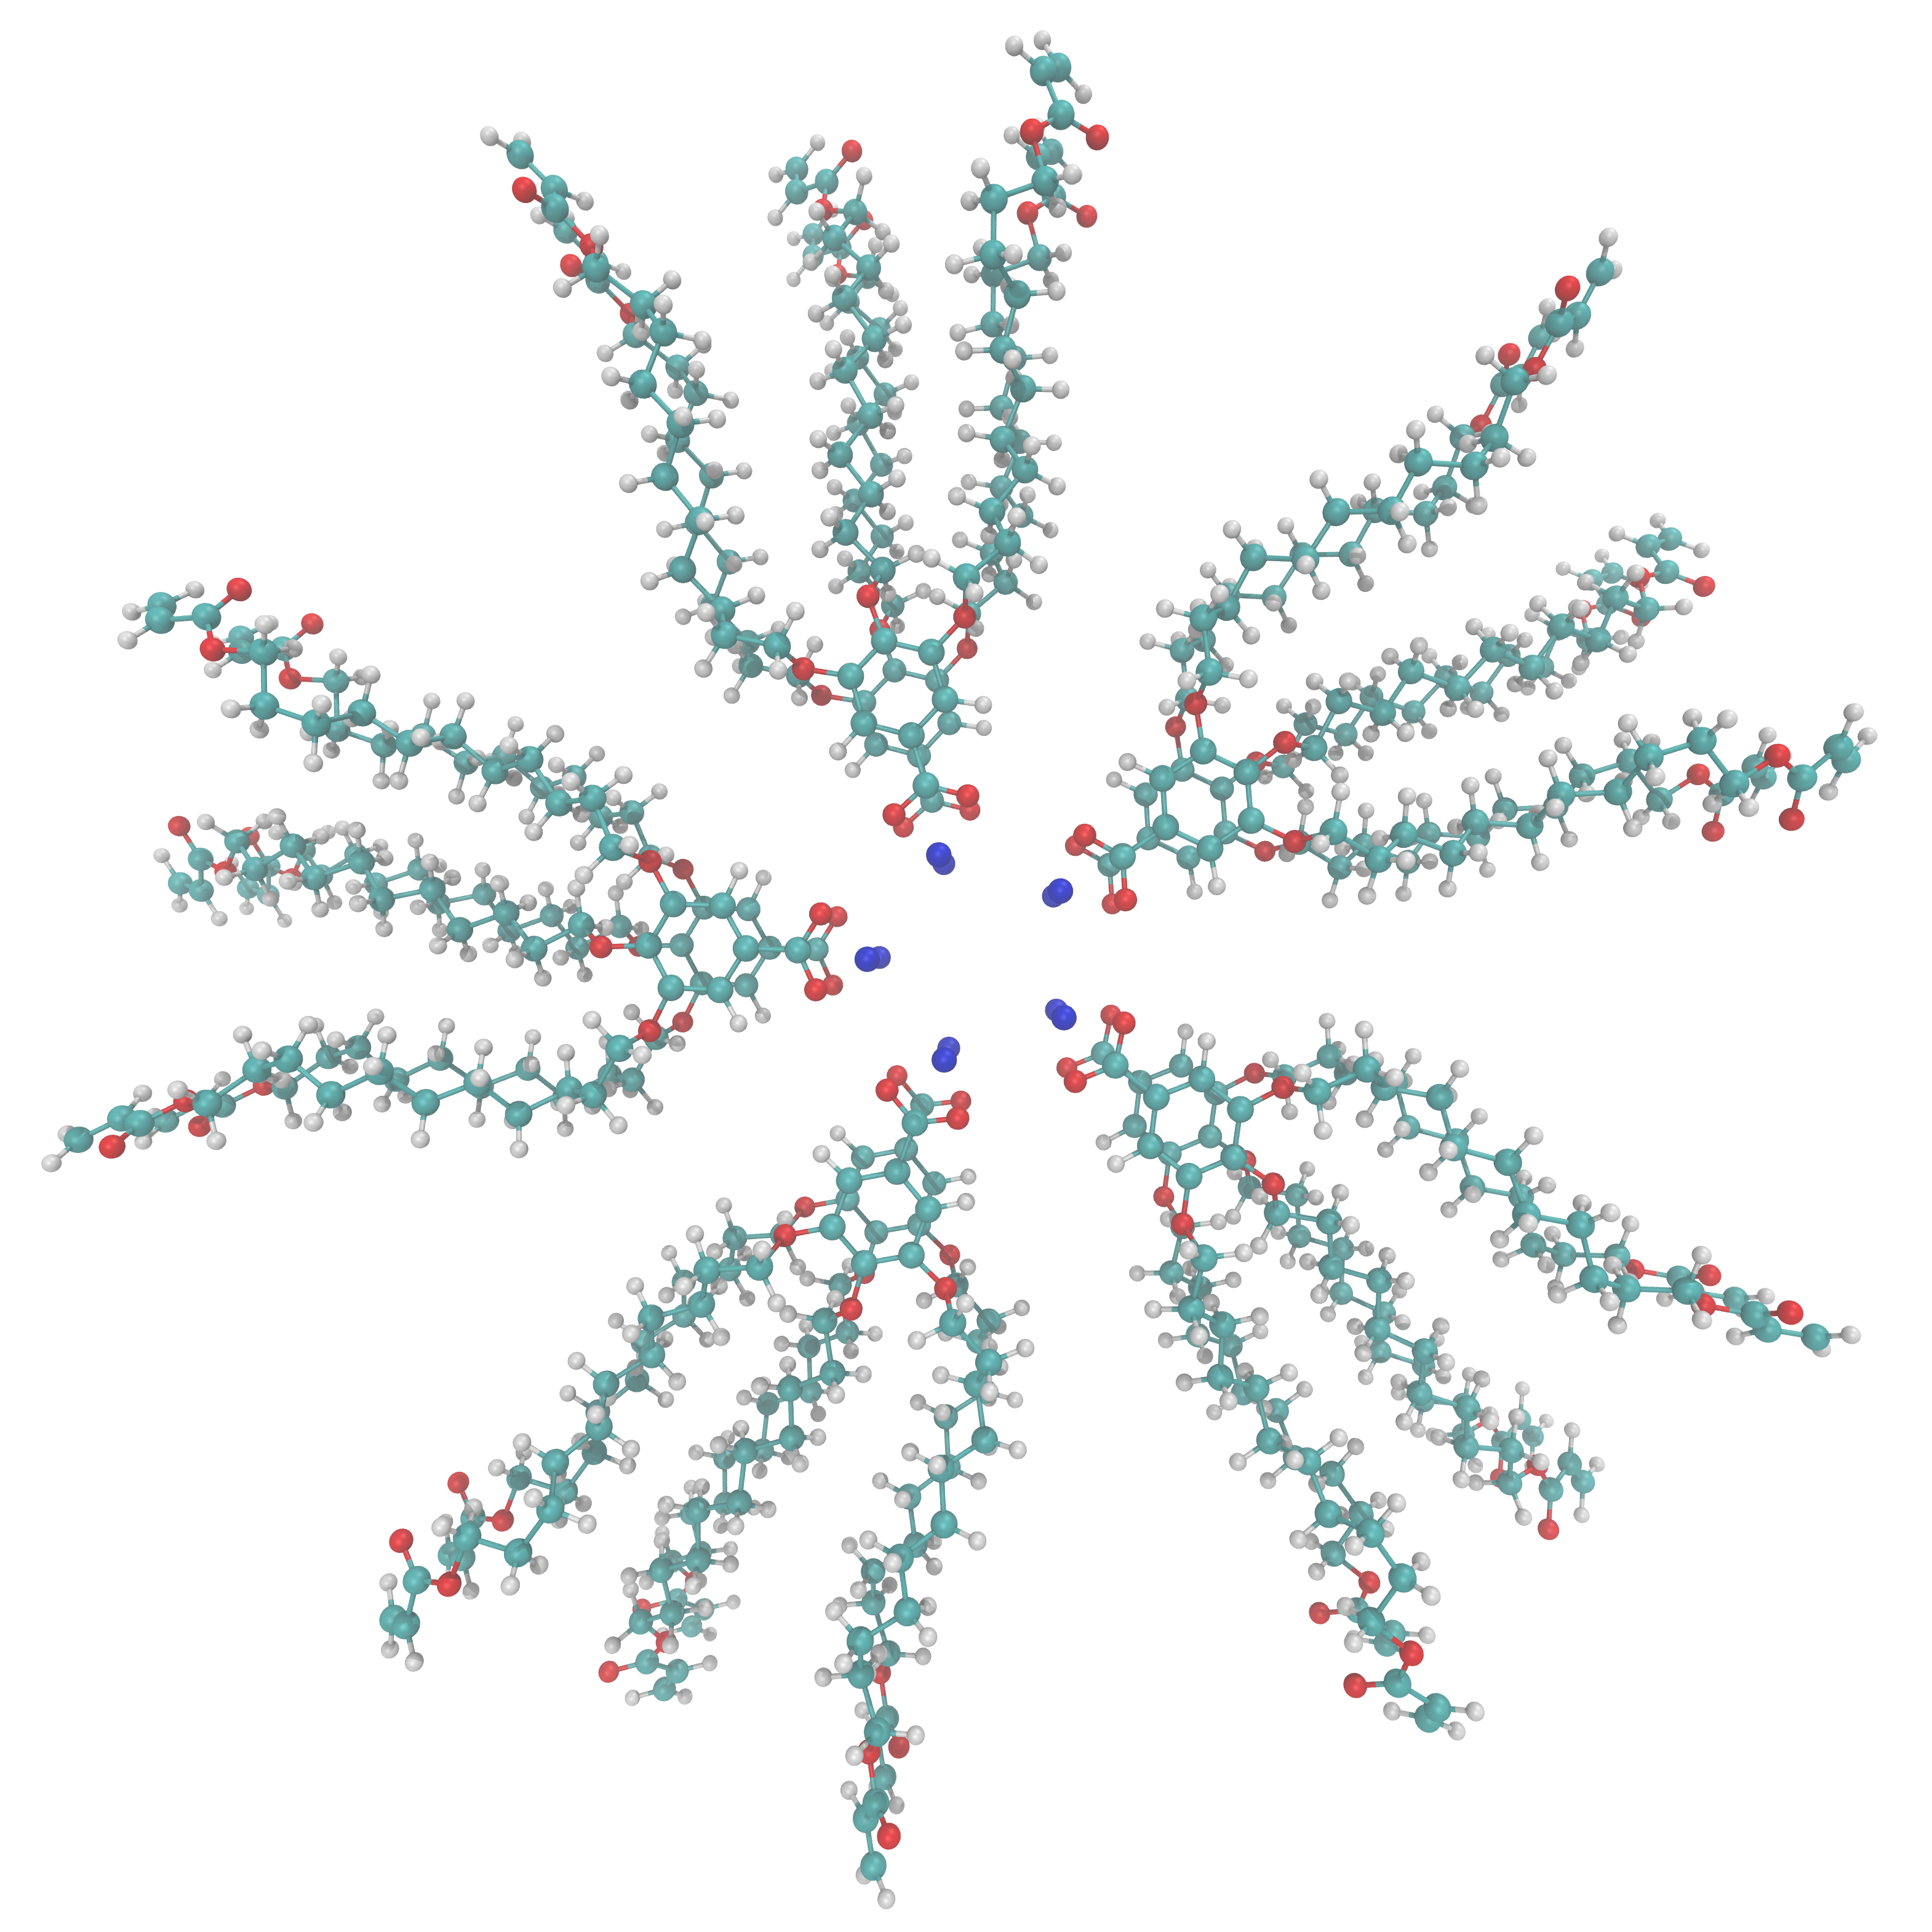
\includegraphics[width=\textwidth]{sandwichedlayers.png}
                \caption{Sandwiched}\label{fig:sandwichedlayers}
        \end{subfigure}
        \begin{subfigure}{0.475\textwidth}
                \centering
                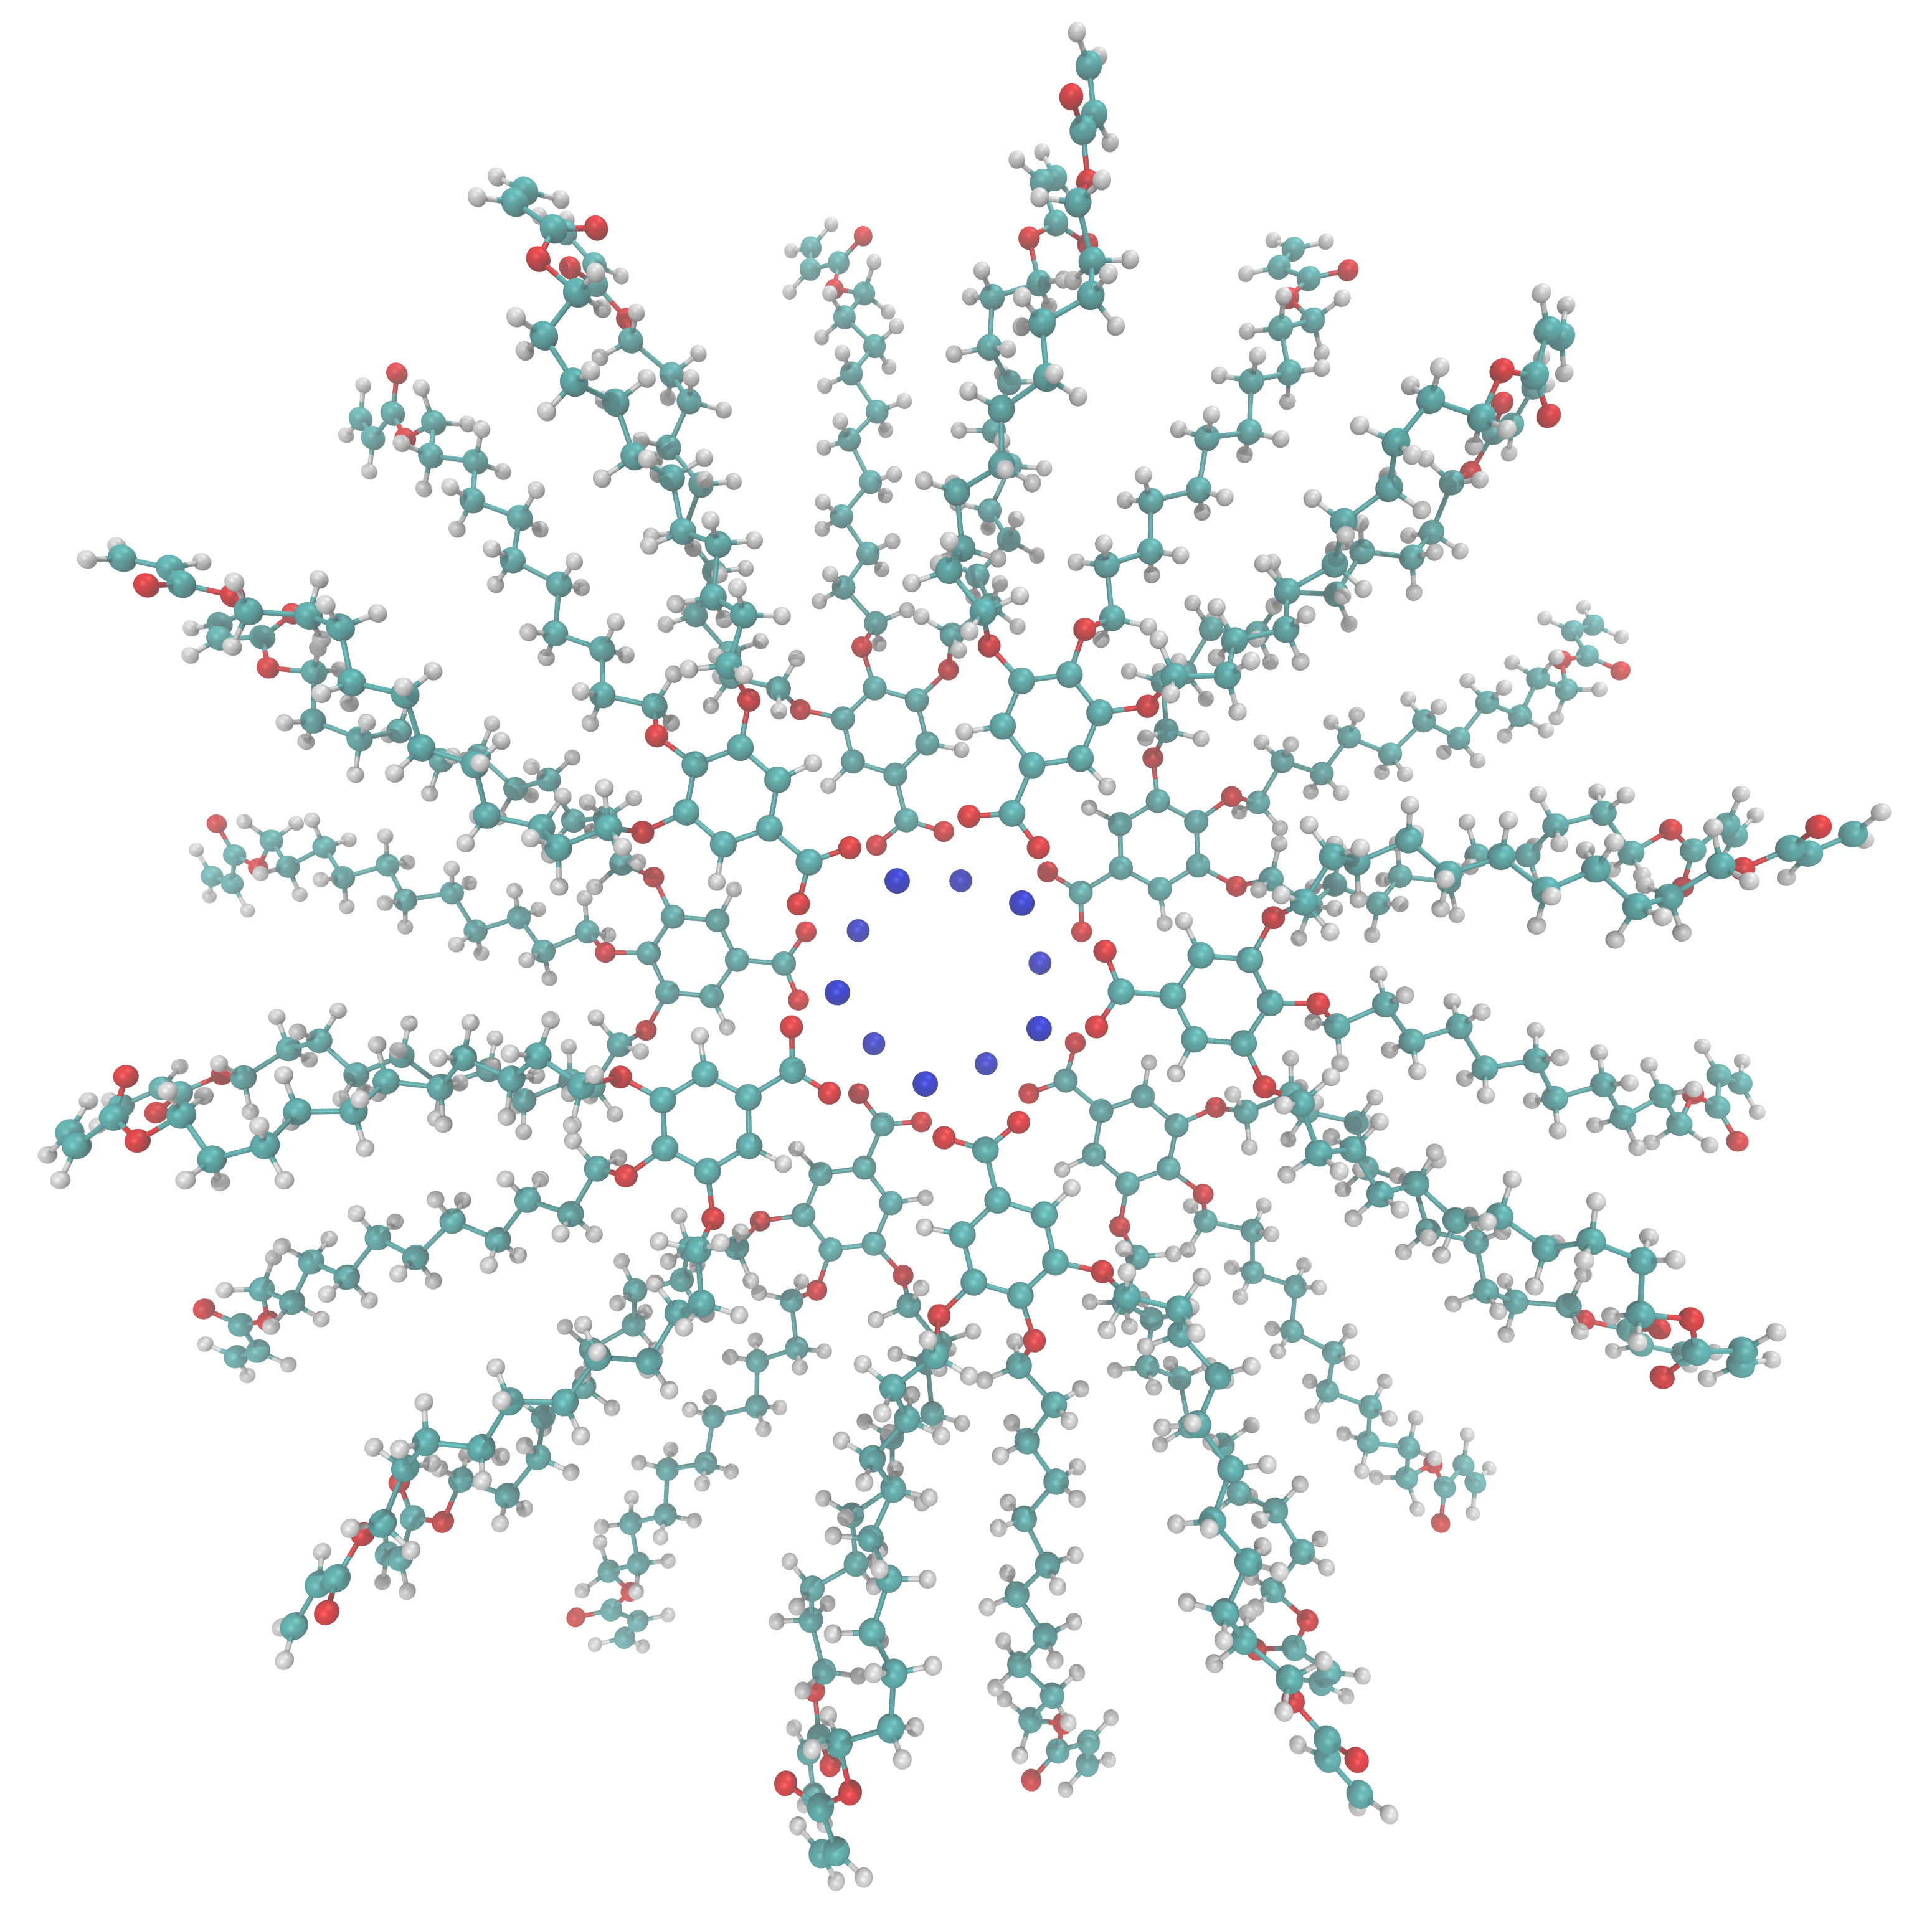
\includegraphics[width=\textwidth]{offsetlayers.png}
                \caption{Parallel Displaced}\label{fig:offsetlayers}
        \end{subfigure}
	\caption{}\label{fig:initial_configs}
\end{figure}

\begin{figure}
        \begin{subfigure}{0.33\textwidth}
                \centering
                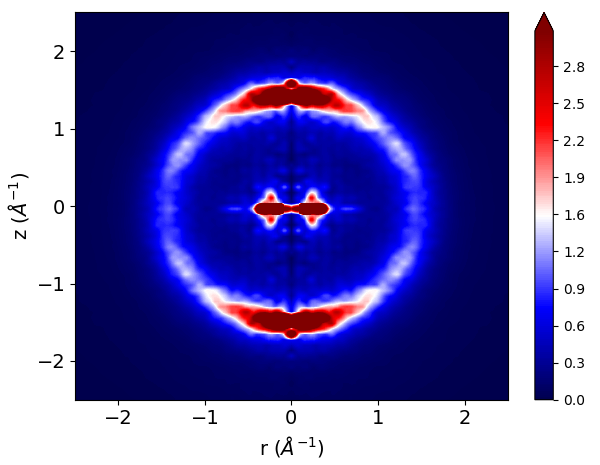
\includegraphics[width=\textwidth]{rzplot_layered_300K.png}
                \caption{Sandwiched}\label{fig:xrd_layered}
        \end{subfigure}
        \begin{subfigure}{0.33\textwidth}
                \centering
                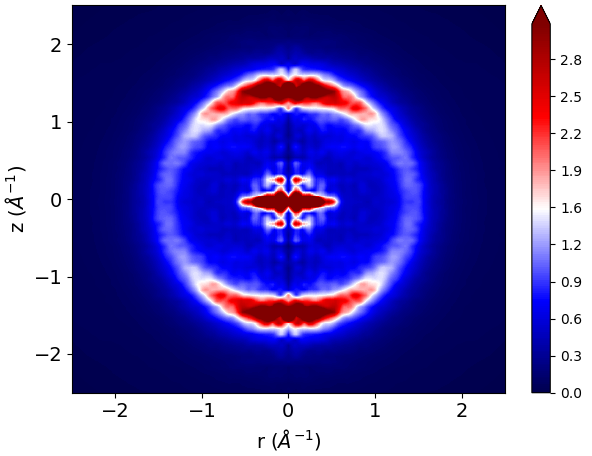
\includegraphics[width=\textwidth]{rzplot_offset_300K.png}
                \caption{Parallel Displaced}\label{fig:xrd_offset}
        \end{subfigure}
	\begin{subfigure}{0.33\textwidth}
                \centering
                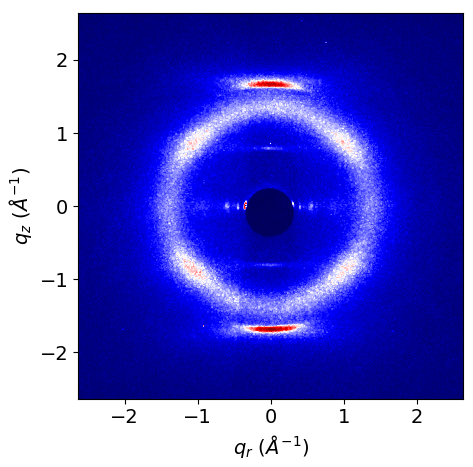
\includegraphics[width=\textwidth]{WAXS_raw.png}
                \caption{Experiment}\label{fig:xrd_exp}
        \end{subfigure}
	\caption{}\label{fig:xrd}
\end{figure}

\begin{figure}
        \begin{subfigure}{0.475\textwidth}
                \centering
                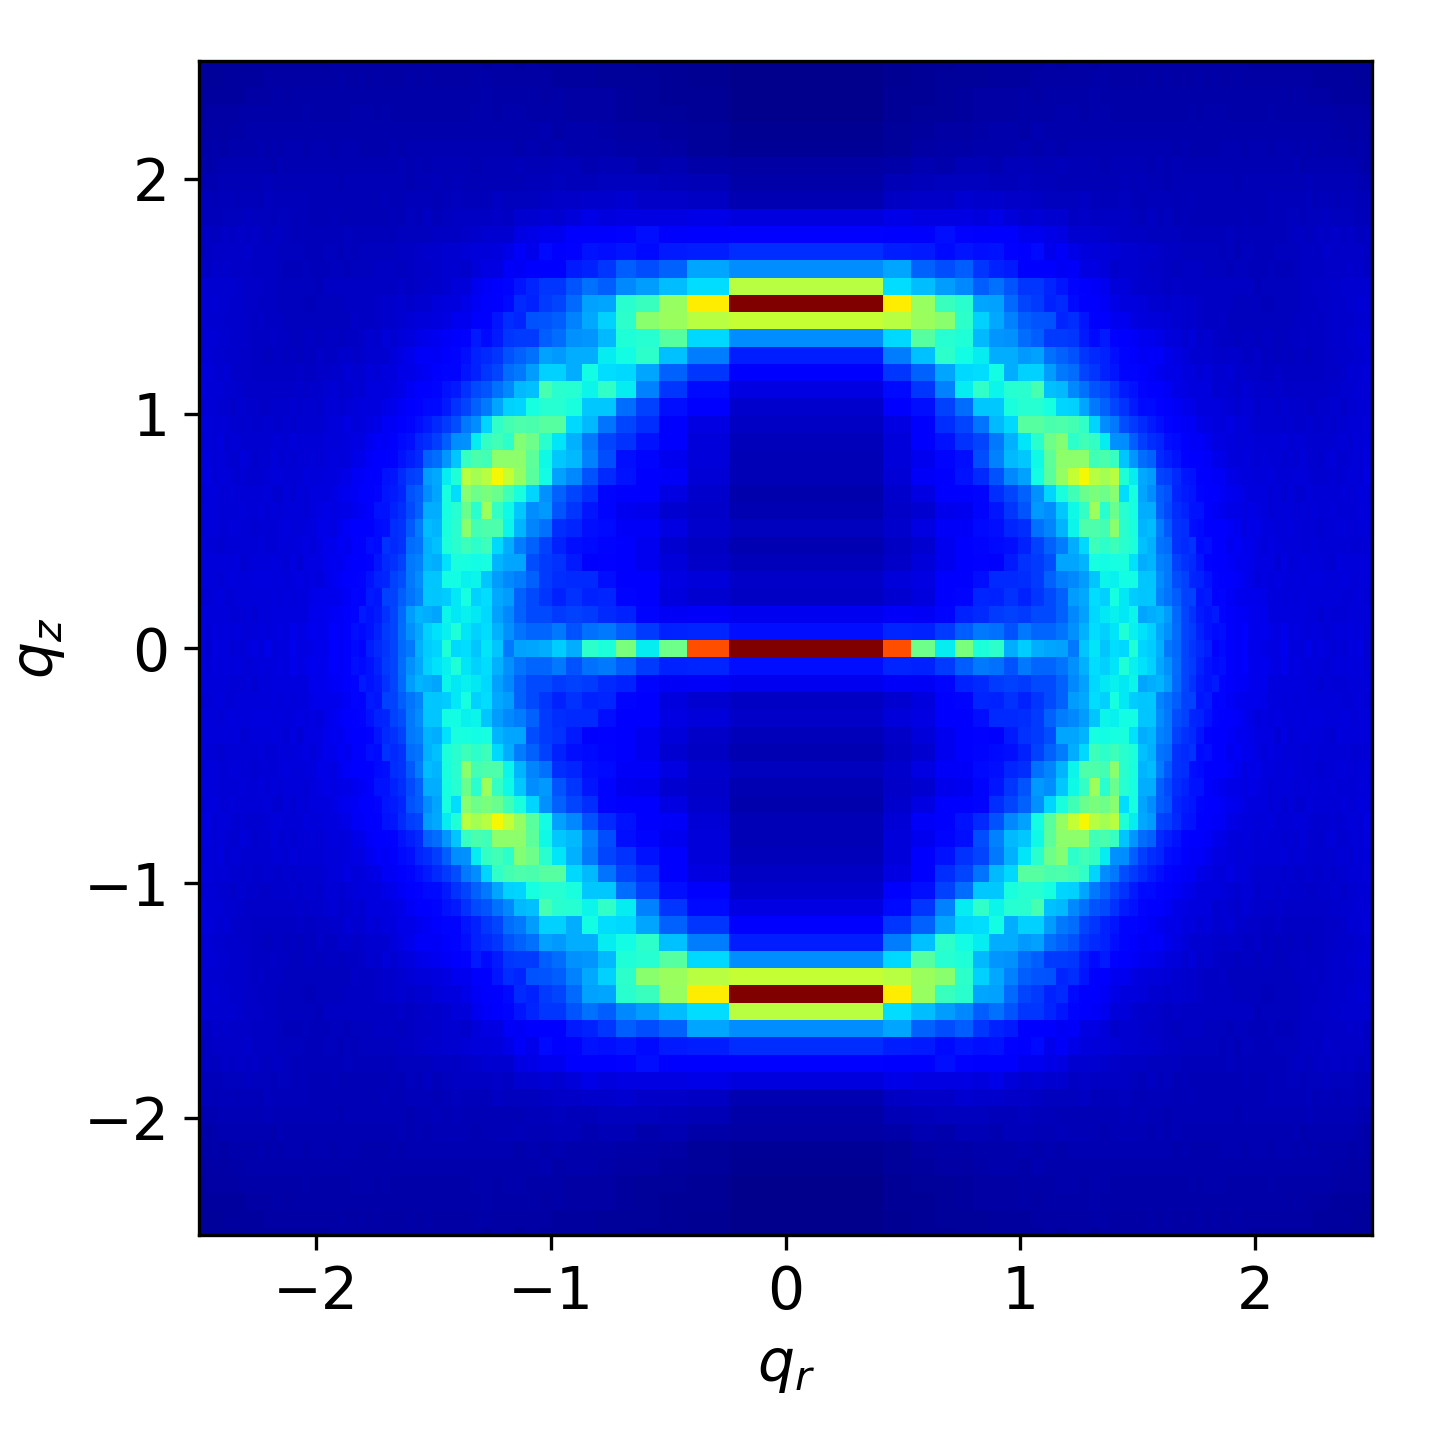
\includegraphics[width=\textwidth]{layered_rzplot.png}
                \caption{Sandwiched}\label{fig:xrd_layered}
        \end{subfigure}
        \begin{subfigure}{0.475\textwidth}
                \centering
                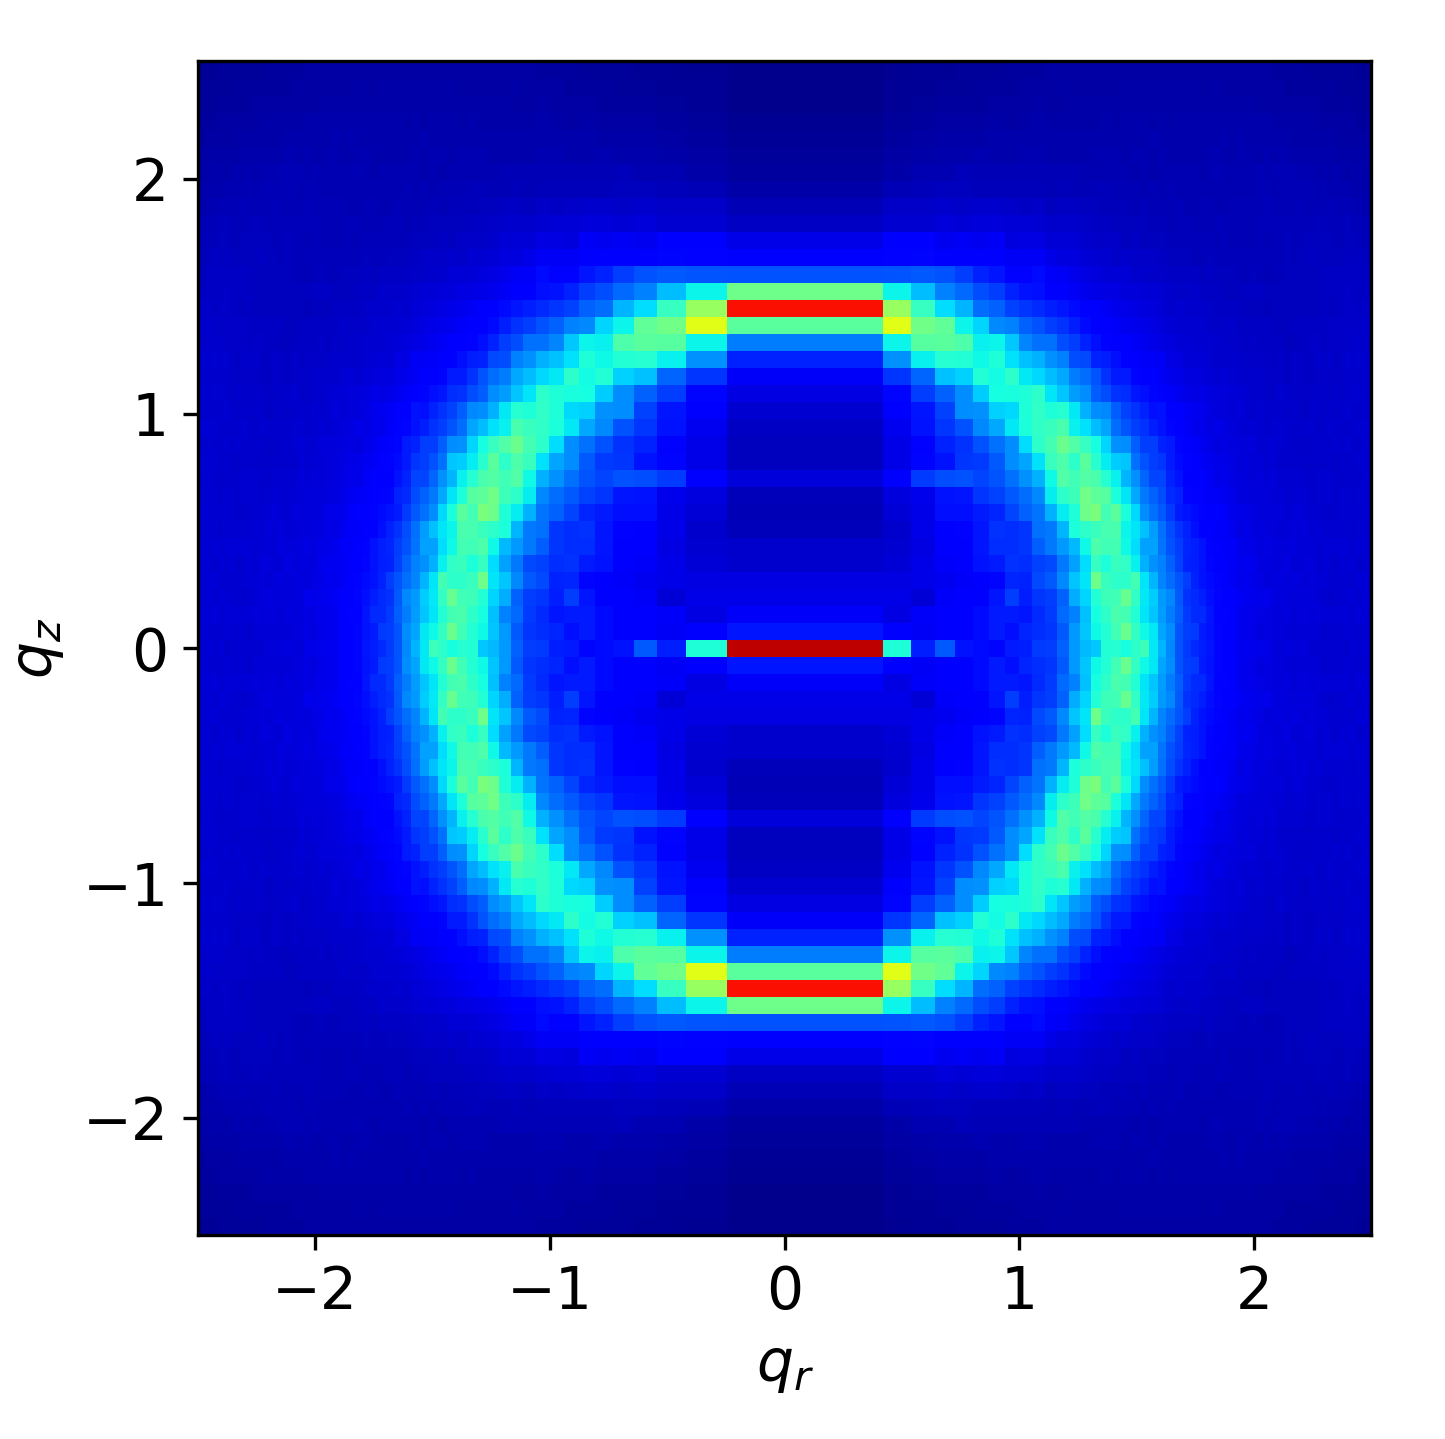
\includegraphics[width=\textwidth]{offset_rzplot.png}
                \caption{Parallel Displaced}\label{fig:xrd_offset}
        \end{subfigure}
	\caption{}\label{fig:xrd_280}
\end{figure}

The hypothesis is that the subharmonic appears due to the reflection located at
($q_r=0,q_z$=1.7) in the experimental pattern. This reflection likely appears
because aromatic rings of monomer head groups pi-stack on top of each other
3.7~\AA apart. The subharmonic does not appear in our simulated patterns and
we need a good explanation for why that is the case. I explored fourier
transforms in various dimensions to help increase my understanding.
  
I first looked at the 1D case. I spaced delta functions 3.7 units (I'll call
the units angstroms for simplicity) apart. I adjusted the real space resolution
by increasing the number of points between delta functions. 

\begin{figure}
        \begin{subfigure}{0.33\textwidth}
                \centering
                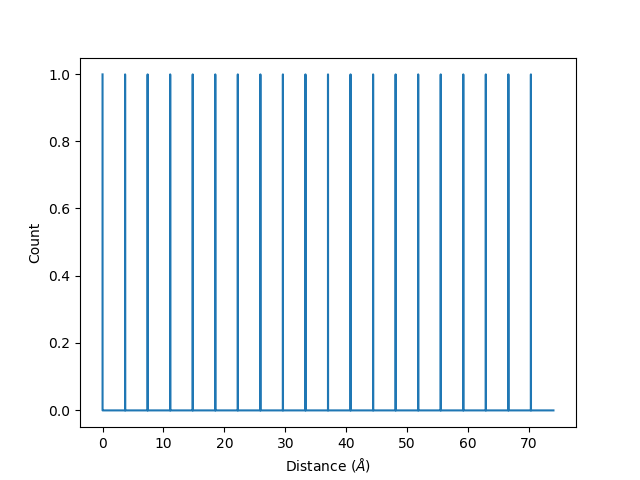
\includegraphics[width=\textwidth]{real_delta_1d_highres.png}
                \caption{Real space - high resolution}\label{fig:real_delta_1d_highres}
        \end{subfigure}
        \begin{subfigure}{0.33\textwidth}
                \centering
                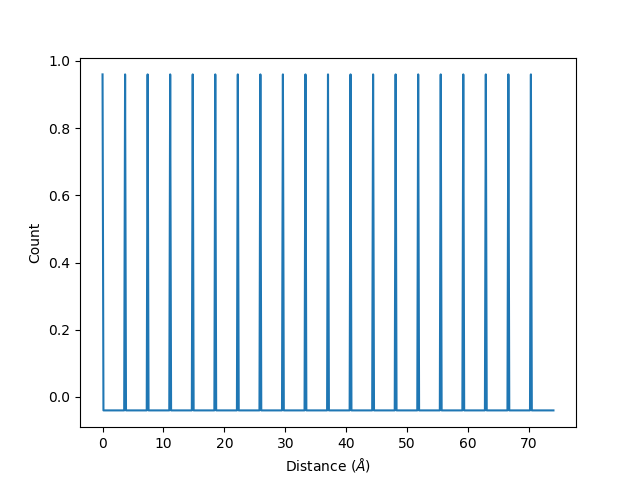
\includegraphics[width=\textwidth]{real_delta_1d_medres.png}
                \caption{Real space - medium resolution}\label{fig:real_delta_1d_medres}
        \end{subfigure}
	\begin{subfigure}{0.33\textwidth}
                \centering
                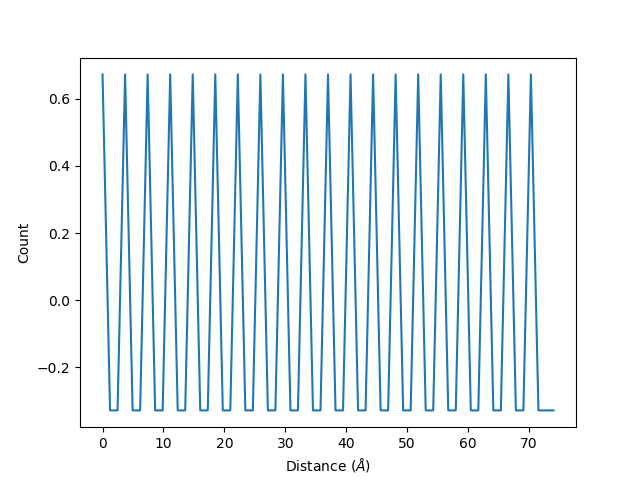
\includegraphics[width=\textwidth]{real_delta_1d_lowres.png}
                \caption{Real space - low resolution}\label{fig:real_delta_1d_lowres}
	\end{subfigure}
        \begin{subfigure}{0.33\textwidth}
                \centering
                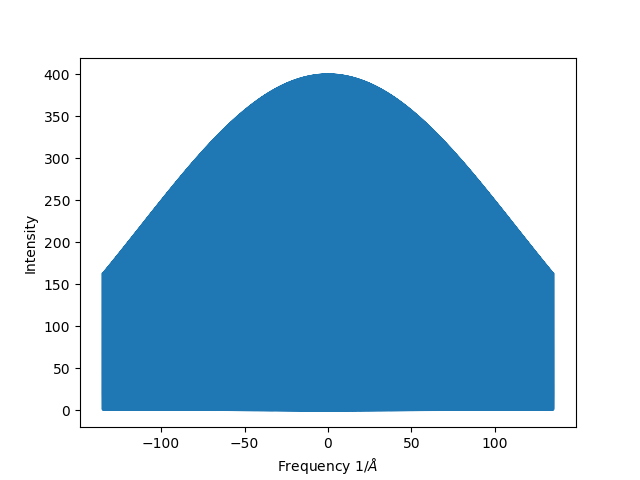
\includegraphics[width=\textwidth]{fourier_delta_1d_highres.png}
                \caption{Fourier space - high resolution}\label{fourier_delta_1d_highres}
        \end{subfigure}
        \begin{subfigure}{0.33\textwidth}
                \centering
                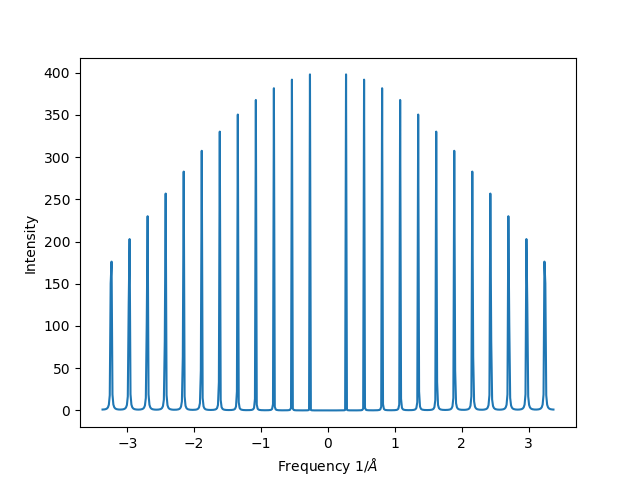
\includegraphics[width=\textwidth]{fourier_delta_1d_medres}
                \caption{Fourier space - medium resolution}\label{fourier_delta_1d_medres}
        \end{subfigure}
        \begin{subfigure}{0.33\textwidth}
                \centering
                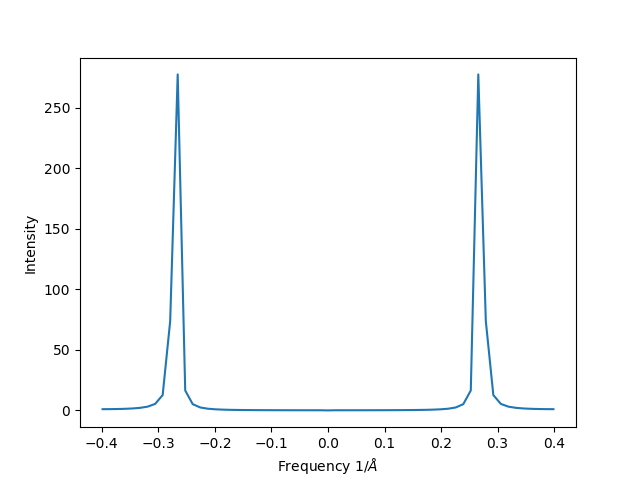
\includegraphics[width=\textwidth]{fourier_delta_1d_lowres}
                \caption{Fourier space - low resolution}\label{fourier_delta_1d_lowres}
        \end{subfigure}
	\caption{Less subharmonics are present as resolution decreases}\label{fig:1D_deltas}
\end{figure}

Next, I replaced the delta function with gaussian functions. It turns out, the
number of subharmonics is dependent on the real space resolution and the width
of the gaussian. A larger sigma value leads to less subharmonics
(Figure~\ref{fig:1D_fourier_sigma}). The same trend seen in
Figure~\ref{fig:1D_deltas} is observed as real space resolution is increased
for a given sigma. That is, more subharmonics appear as resolution increases.
In the context of stacked benzene rings I would expect a more disordered system
to have less subharmonics. It is also possible to miss out on subharmonics if
the real space resolution is too small (i.e. data is binned into too large of
bins). 

None of these subharmonics would actually show up in the experimental pattern
(except maybe the first one) because the wavelength of the X-rays is too large
(1.54 \AA). And there are no subharmonics corresponding to a real space
separation greater than 3.7 \AA. In order for the 7.4 \AA reflection to show
up, rings need to be spaced 7.4 \AA vertically. Then there would be a 3.7 \AA
subharmonic which shows up as the $\pi$-stacking reflection. In all plots,
subharmonics are always weaker in intensity than the fundamental frequency. 
So the question remains, why is the $\pi$-stacking reflection stronger than
the 7.4 \AA reflection? 

\begin{figure}
        \begin{subfigure}{0.33\textwidth}
                \centering
                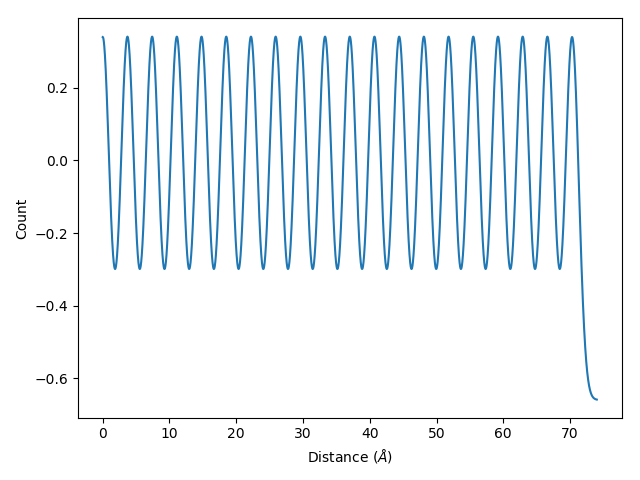
\includegraphics[width=\textwidth]{real_gauss_1d_highsig.png}
                \caption{Real space - sigma = 1}\label{fig:real_gauss_1d_highsig}
        \end{subfigure}
        \begin{subfigure}{0.33\textwidth}
                \centering
                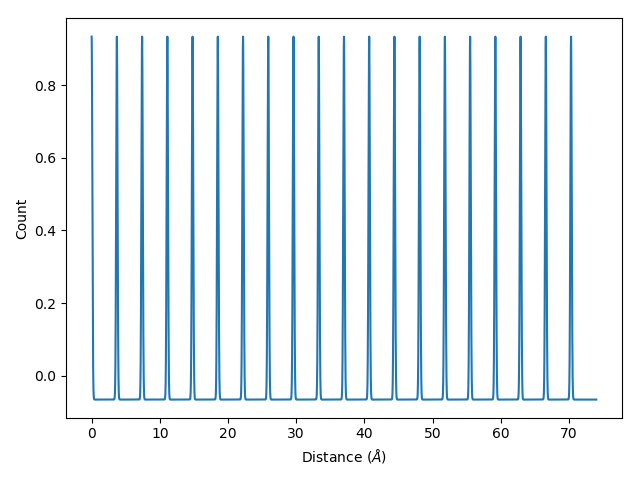
\includegraphics[width=\textwidth]{real_gauss_1d_medsig.png}
                \caption{Real space - sigma = 0.1}\label{fig:real_gauss_1d_medsig}
        \end{subfigure}
	\begin{subfigure}{0.33\textwidth}
                \centering
                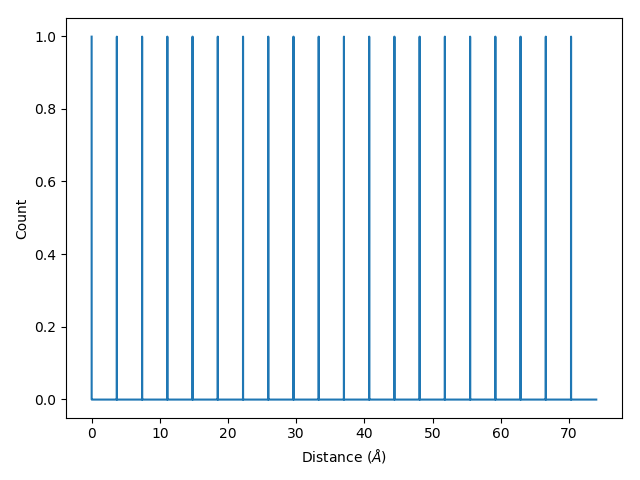
\includegraphics[width=\textwidth]{real_gauss_1d_lowsig.png}
                \caption{Real space - sigma = 0.001}\label{fig:real_gauss_1d_lowsig}
	\end{subfigure}
        \begin{subfigure}{0.33\textwidth}
                \centering
                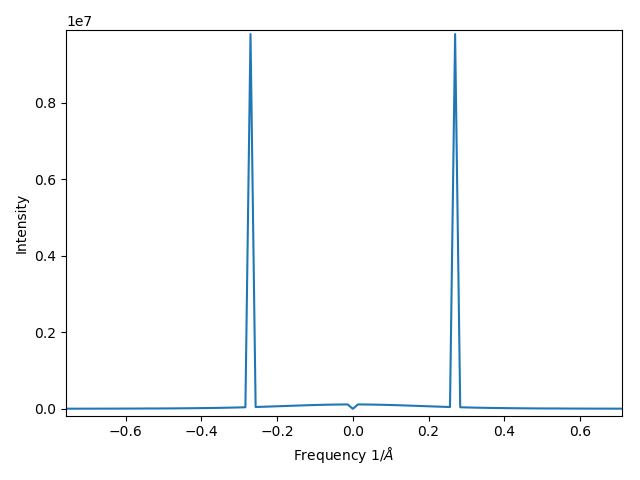
\includegraphics[width=\textwidth]{fourier_gauss_1d_highsig.png}
                \caption{Fourier space - sigma = 1}\label{fourier_gauss_1d_highsig}
        \end{subfigure}
        \begin{subfigure}{0.33\textwidth}
                \centering
                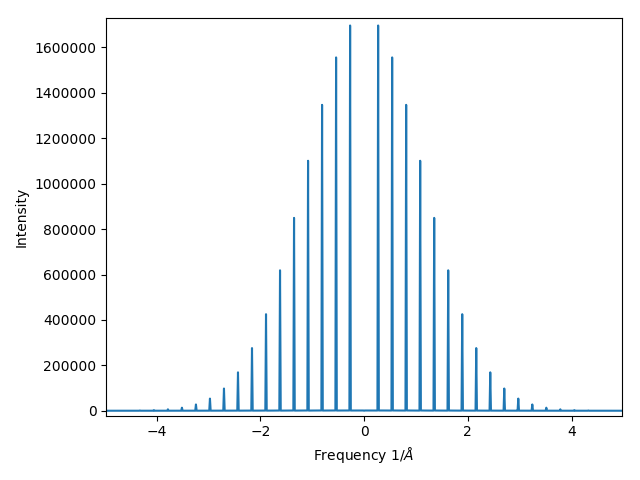
\includegraphics[width=\textwidth]{fourier_gauss_1d_medsig}
                \caption{Fourier space - sigma = 0.1}\label{fourier_gauss_1d_medsig}
        \end{subfigure}
        \begin{subfigure}{0.33\textwidth}
                \centering
                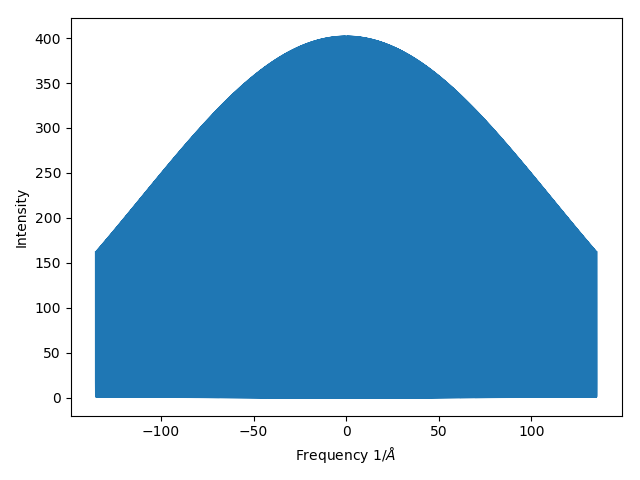
\includegraphics[width=\textwidth]{fourier_gauss_1d_lowsig}
                \caption{Fourier space - sigma = 0.001}\label{fourier_gauss_1d_lowsig}
        \end{subfigure}
	\caption{Using high real space resolution (same as Figure~\ref{1D_deltas}), it
                 is evident that a smaller sigma leads to more subharmonics. As sigma
		 approaches zero, the behavior is the fourier transform resembles that
		 of delta functions. Otherwise, the fourier transform of a gaussian is
		 a gaussian.}\label{fig:1D_gauss_sigma}
\end{figure}

Next, I explored 2D fourier transforms of grids of data that somewhat resemble 
the LLC system. I created parallel columns of points spaced 3.7\AA~apart. Each
point is represented as a 2-dimensional gaussian function. In Figure~\ref{fig:2d_columns_simple}
I show examples of simple configurations made up of one and two columns. 

\begin{figure}
	\begin{subfigure}{0.45\textwidth}
	        \centering
                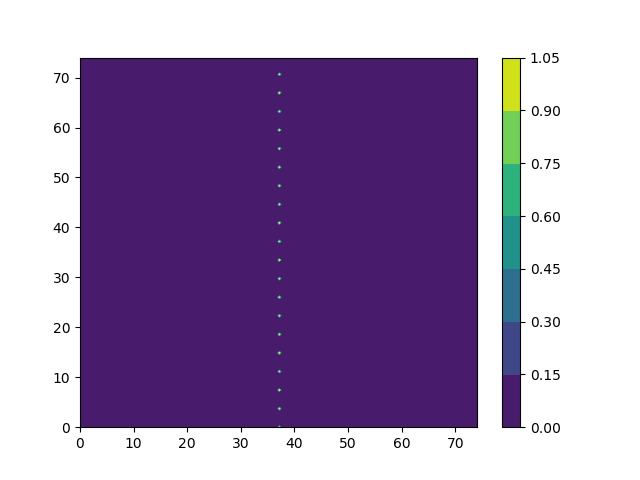
\includegraphics[width=\textwidth]{real_2d_1column.png}
                \caption{Real space - $\sigma_x=\sigma_y$ = 0.001}\label{fig:real_2d_1column}
        \end{subfigure}
        \begin{subfigure}{0.45\textwidth}
                \centering
                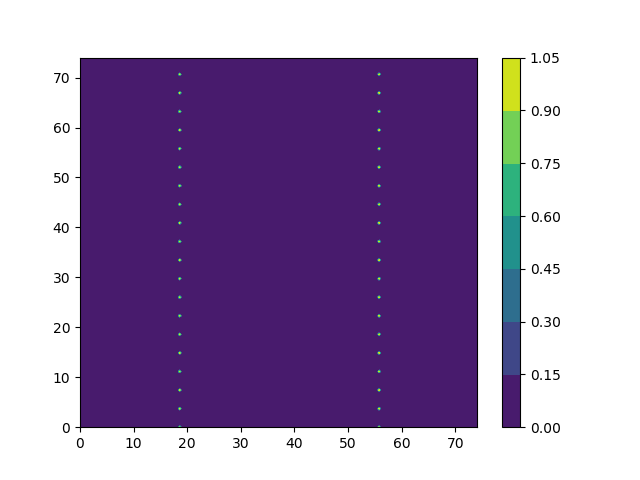
\includegraphics[width=\textwidth]{real_2d_2column.png}
                \caption{Real space - $\sigma_x=\sigma_y$ = 0.001}\label{fig:real_2d_2column}
        \end{subfigure}
	\begin{subfigure}{0.45\textwidth}
                \centering
                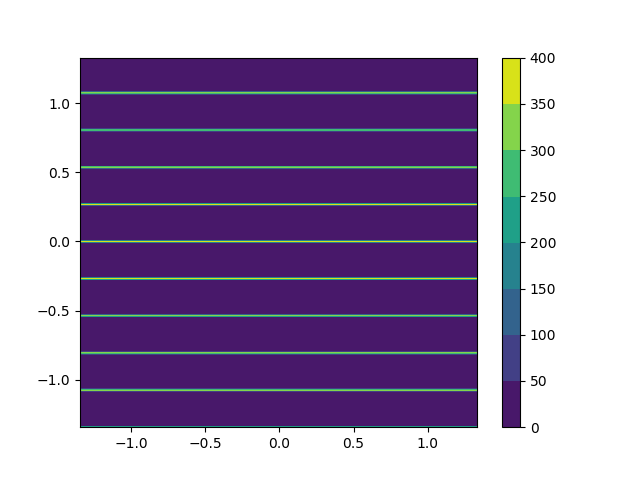
\includegraphics[width=\textwidth]{fourier_2d_1column.png}
                \caption{Fourier space}\label{fig:fourier_2d_1column}
	\end{subfigure}
        \begin{subfigure}{0.45\textwidth}
                \centering
                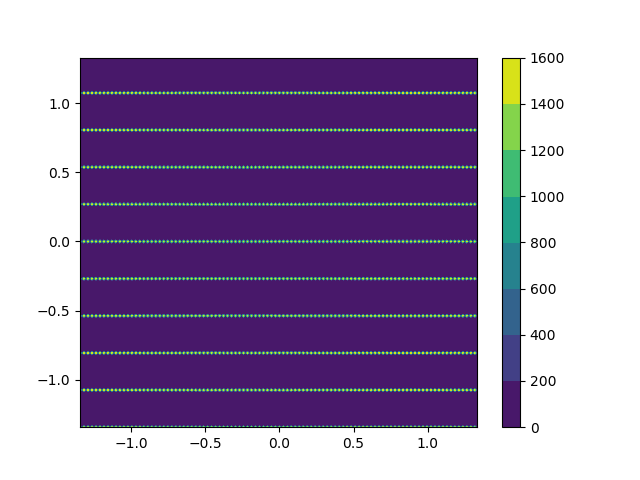
\includegraphics[width=\textwidth]{fourier_2d_2column.png}
                \caption{Fourier space}\label{fourier_2d_2column}
        \end{subfigure}
	\caption{A single column of equispaced scatterers shows up as horizontal lines
		 with spacing equal to the inverse of the distance between scatters. Adding
		 a second column (b) causes the horizontal lines to become dots spaced apart
		 by the inverse of the distance between columns. Adding more columns would
                 follow the same trend.}~\label{fig:2d_columns_simple}
\end{figure}

Next, I explored columns with points spaced 7.4 \AA apart.
Figure~\ref{fig:2d_columns_offset} shows the fourier transform of a single
column. In Figure~\ref{fig:fourier_2d_74_1column} we see that the intensity of
each parallel line is about the same. Recall that the line corresponding to the
fundamental frequency (7.4 \AA real space) needs to be weaker in intensity than
its first subharmonic in order to be consistent with experiment. Turns out, we
can choose values of $\sigma_x$ and $\sigma_y$ that make this happen. If we 
change $\sigma_y$=0.4, we observe a faded effect at high frequency values. In this
way we would observe the $\pi$-stacking reflection as more intense than the 
7.4\AA reflection. It is also important that $\sigma_x$ stays low, otherwise, the
reflection disappears from the middle (Figure~\ref{fig:fourier_2d_74_1column_highxysig}). 

\begin{figure}
	\begin{subfigure}{0.45\textwidth}
                \centering
                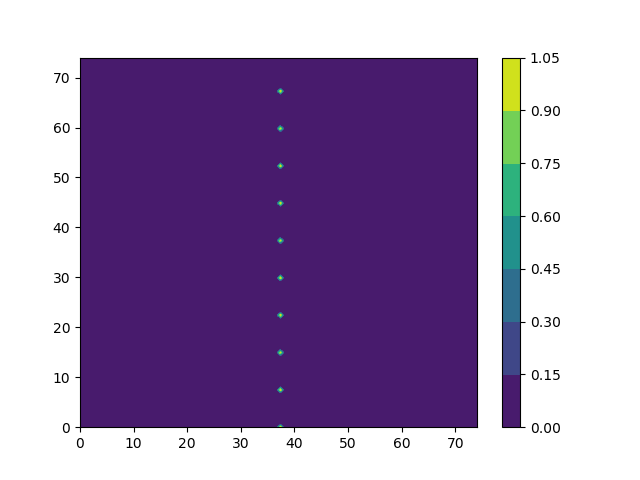
\includegraphics[width=\textwidth]{real_2d_74_1column.png}
                \caption{Real space - $\sigma_x$=$\sigma_y$=0.1}\label{fig:real_2d_74_1column}
        \end{subfigure}
        \begin{subfigure}{0.45\textwidth}
                \centering
                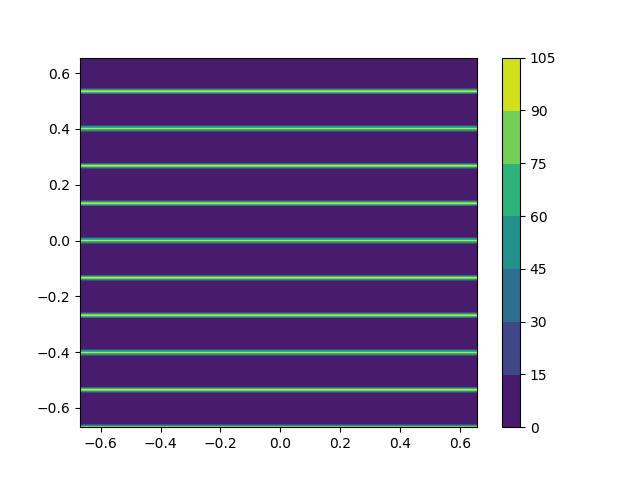
\includegraphics[width=\textwidth]{fourier_2d_74_1column.png}
                \caption{Fourier space}\label{fig:fourier_2d_74_1column}
        \end{subfigure}
	\begin{subfigure}{0.45\textwidth}
                \centering
                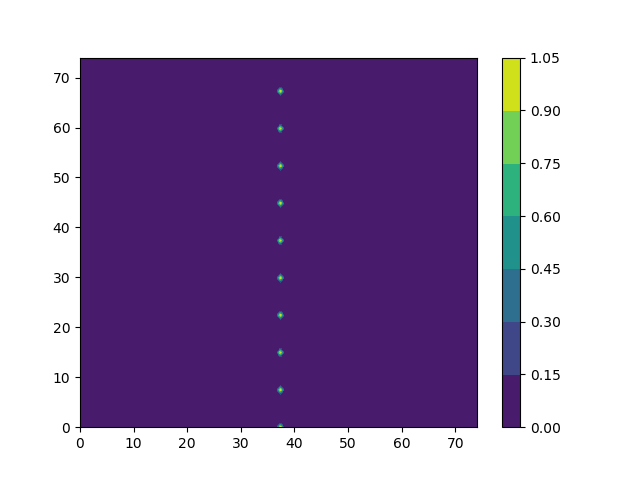
\includegraphics[width=\textwidth]{real_2d_74_1column_highysig.png}
                \caption{Real space - $\sigma_x$=0.1, $\sigma_y$=0.4}\label{fig:real_2d_74_1column_highysig}
        \end{subfigure}
        \begin{subfigure}{0.45\textwidth}
                \centering
                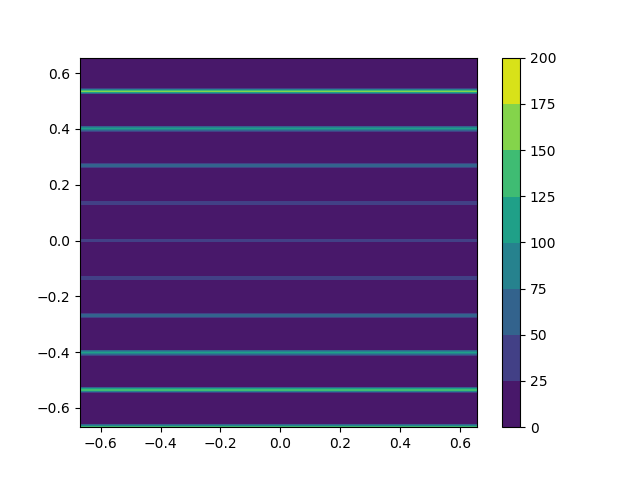
\includegraphics[width=\textwidth]{fourier_2d_74_1column_highysig.png}
                \caption{Fourier space}\label{fig:fourier_2d_74_1column_highysig}
        \end{subfigure}
	\begin{subfigure}{0.45\textwidth}
                \centering
                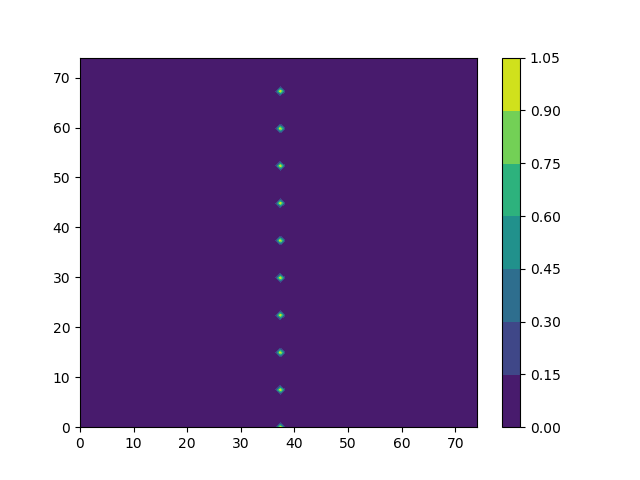
\includegraphics[width=\textwidth]{real_2d_1column_74_highxysig.png}
                \caption{Real space - $\sigma_x$=0.4, $\sigma_y$=0.4}\label{fig:real_2d_1column_75_highxysig}
        \end{subfigure}
        \begin{subfigure}{0.45\textwidth}
                \centering
                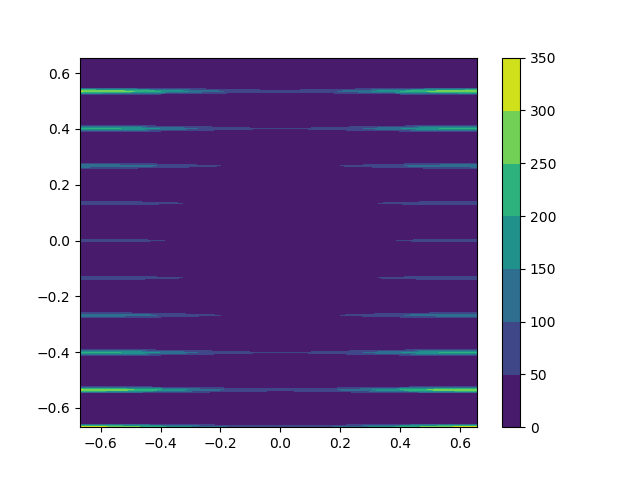
\includegraphics[width=\textwidth]{fourier_2d_1column_74_highxysig.png}
                \caption{Fourier space}\label{fig:fourier_2d_74_1column_highxysig}
        \end{subfigure}

        \caption{A single column of scatterers spaced 7.4 \AA apart shows up as horizontal lines
                 with spacing equal to the inverse of the distance between scatters. One of the
                 subharmonics corresponds to a real spacing distance of 3.7 \AA. If we adjust the 
	         sigmas of the scattering, we can change the relative intensity of each
                 horizontal line in fourier space.}~\label{fig:2d_columns_offset}
\end{figure}

 
\end{document}
